\documentclass[conference]{IEEEtran}
\IEEEoverridecommandlockouts
\usepackage[T1]{fontenc}
\usepackage[utf8]{inputenc}
\usepackage{cite}
\usepackage{amsmath,amssymb}
\usepackage{graphicx}
\usepackage{booktabs}
\usepackage{array}
\usepackage{microtype}
\usepackage{textcomp}
\usepackage{url}
\usepackage{float}

\hyphenation{multi-plier look-ahead}

\begin{document}

\title{Design and Verification of a Parameterized SIMD\\Vector Processing Unit in Verilog}

\author{%
\begin{tabular*}{\textwidth}{@{\extracolsep{\fill}}cccc}
Mohammed Yaseen & Palwai Tejaswini & Nishant Ranjan Singh & Sankalp M Tellur\\
{\small Roll No.\ 2401010281} & {\small Roll No.\ 2401010314} & {\small Roll No.\ 2401010301} & {\small Roll No.\ 2401010416}
\end{tabular*}\\[1.8ex]
\textit{Modern Computer Architecture}%
}

\maketitle

\begin{abstract}
This paper presents the design and evaluation of a parameterized SIMD Vector Processing Unit (VPU) implemented in Verilog. The VPU supports a configurable 1--16 lane count, eight vector registers, a 16-opcode vector instruction set and a strip-mining loop instruction. The same one-lane configuration provides the scalar cycle-count baseline. Four workloads were simulated at five lane counts, giving 20 saved system runs with zero output errors; a separate lane-ALU test records 19 passing directed cases. For vector addition, the four-lane configuration takes 81 cycles compared with 321 cycles for one lane, a measured cycle-count speed-up of 3.96$\times$. Saved Yosys reports provide preliminary mapping statistics for selected modules only. No top-level FPGA implementation or maximum-frequency measurement is available, so hardware timing and whole-device utilization are not claimed.
\end{abstract}

\begin{IEEEkeywords}
SIMD, vector processor, data-level parallelism, Verilog HDL, RTL verification, FPGA, computer architecture.
\end{IEEEkeywords}

%=====================================================================
\section{Introduction}
Single Instruction, Multiple Data (SIMD) execution applies one instruction to several data elements at once and is the most common way processors exploit data-level parallelism~\cite{flynn1966}. It appears in historic vector supercomputers~\cite{russell1978}, in subword-parallel multimedia extensions~\cite{peleg1996,lee1996}, in contemporary vector ISAs such as ARM SVE~\cite{stephens2017} and the RISC-V Vector extension~\cite{rvv2021}, and in the tensor and matrix engines used for AI workloads. Understanding SIMD therefore connects directly to the course topics on instruction-level and data-level parallelism, memory systems and modern AI hardware.

This project implements a compact SIMD Vector Processing Unit in Verilog with a vector register file, lane-parallel ALUs, vector control, arithmetic and logical instructions, vector memory operations and a hardware loop. The evaluation compares saved cycle counts across lane counts and records selected-module Yosys mapping statistics.

The contributions are: (i)~lane-parameterized VPU RTL with a defined vector ISA; (ii)~a strip-mining loop that advances by the configured lane count; (iii)~an assembler, self-checking testbenches and automation scripts; (iv)~saved cycle-count and speed-up comparisons for four workloads; and (v)~preliminary Yosys mapping reports for selected modules.

%=====================================================================
\section{Literature Review}
\subsection{SIMD and vector architectures}
Flynn's taxonomy classifies SIMD as a distinct class of machine in which a single control stream drives many processing elements~\cite{flynn1966}. The CRAY-1 popularized vector registers and pipelined functional units, showing that long vectors amortize instruction fetch and control overhead~\cite{russell1978}. Espasa et al.\ survey the past and future of vector architectures and argue that they remain attractive for regular, data-parallel code~\cite{espasa1998}, and Asanovi\'c's thesis gives a detailed treatment of vector microprocessor design~\cite{asanovic1998}.

\subsection{Multimedia and modern SIMD extensions}
Commodity processors adopted short-vector SIMD through subword parallelism, in which a wide register is partitioned into several narrow elements. Intel's MMX~\cite{peleg1996} and HP's MAX-2~\cite{lee1996} are early examples. More recently, vector-length-agnostic ISAs such as ARM SVE~\cite{stephens2017} and the RISC-V Vector extension~\cite{rvv2021} let software be written once and run on implementations of different vector width. Our loop instruction follows the same idea at a much smaller scale: the program specifies the total element count and the hardware advances by the implemented lane count.

\subsection{Vector processors in hardware research and on FPGAs}
Academic implementations include the Hwacha vector accelerator~\cite{hwacha2014} and the Ara RISC-V vector processor~\cite{ara2020}, while the data-parallel design trade-offs between programmability and efficiency are explored in~\cite{lee2011}. Soft vector processors for FPGAs, such as VESPA~\cite{vespa2008} and the vector soft-core of Yu et al.~\cite{yu2008}, show that a configurable number of lanes is an effective way to trade area for performance on reconfigurable fabrics. These designs are far larger than a course project, but they motivate our choice of a parameterized lane count.

\subsection{Performance modelling}
Amdahl's law~\cite{amdahl1967} bounds the benefit of parallel hardware by the fraction of work that cannot be parallelized, and the textbook treatment in~\cite{hennessy2017,patterson2020} relates execution time to instruction count, CPI and clock period. We use these relations in Section~\ref{sec:results} to explain the measured speed-up.

\begin{table}[!t]
\caption{Positioning of Related Work}
\label{tab:related}
\centering
\footnotesize
\begin{tabular}{@{}p{1.75cm} p{2.1cm} p{3.4cm}@{}}
\toprule
\textbf{Work} & \textbf{Type} & \textbf{Relevance to this project}\\
\midrule
CRAY-1~\cite{russell1978} & Vector supercomputer & Vector registers, strip-mined loops\\
MMX/MAX-2~\cite{peleg1996,lee1996} & Subword SIMD & Parallel ALU operations on packed data\\
SVE/RVV~\cite{stephens2017,rvv2021} & Scalable vector ISA & Lane-count-independent code\\
VESPA~\cite{vespa2008} & FPGA soft vector CPU & Configurable lanes, FPGA resources\\
\textbf{This work} & Parameterized RTL VPU & Lane-agnostic loop, verified, measured\\
\bottomrule
\end{tabular}
\end{table}

%=====================================================================
\section{Proposed Solution}
\subsection{Architecture overview}
Fig.~\ref{fig:block} shows the proposed VPU. A program counter and an element pointer \textit{ptr} address the instruction memory, which is separate from the data memory (Harvard organization). The vector control unit decodes each 32-bit instruction into a register-write enable, memory read/write strobes, a broadcast select and a loop/halt indication. The vector register file feeds two operand vectors, each $\mathit{LANES}\times 32$ bits wide, to \textit{LANES} identical 32-bit ALUs. A write-back multiplexer selects between the ALU result, a vector loaded from data memory and a broadcast immediate. The number of lanes is a Verilog parameter, so the same source describes the scalar baseline ($\mathit{LANES}=1$) and wider SIMD configurations. The unit executes one instruction per clock cycle (CPI\,=\,1).

\begin{figure*}[!t]
\centering
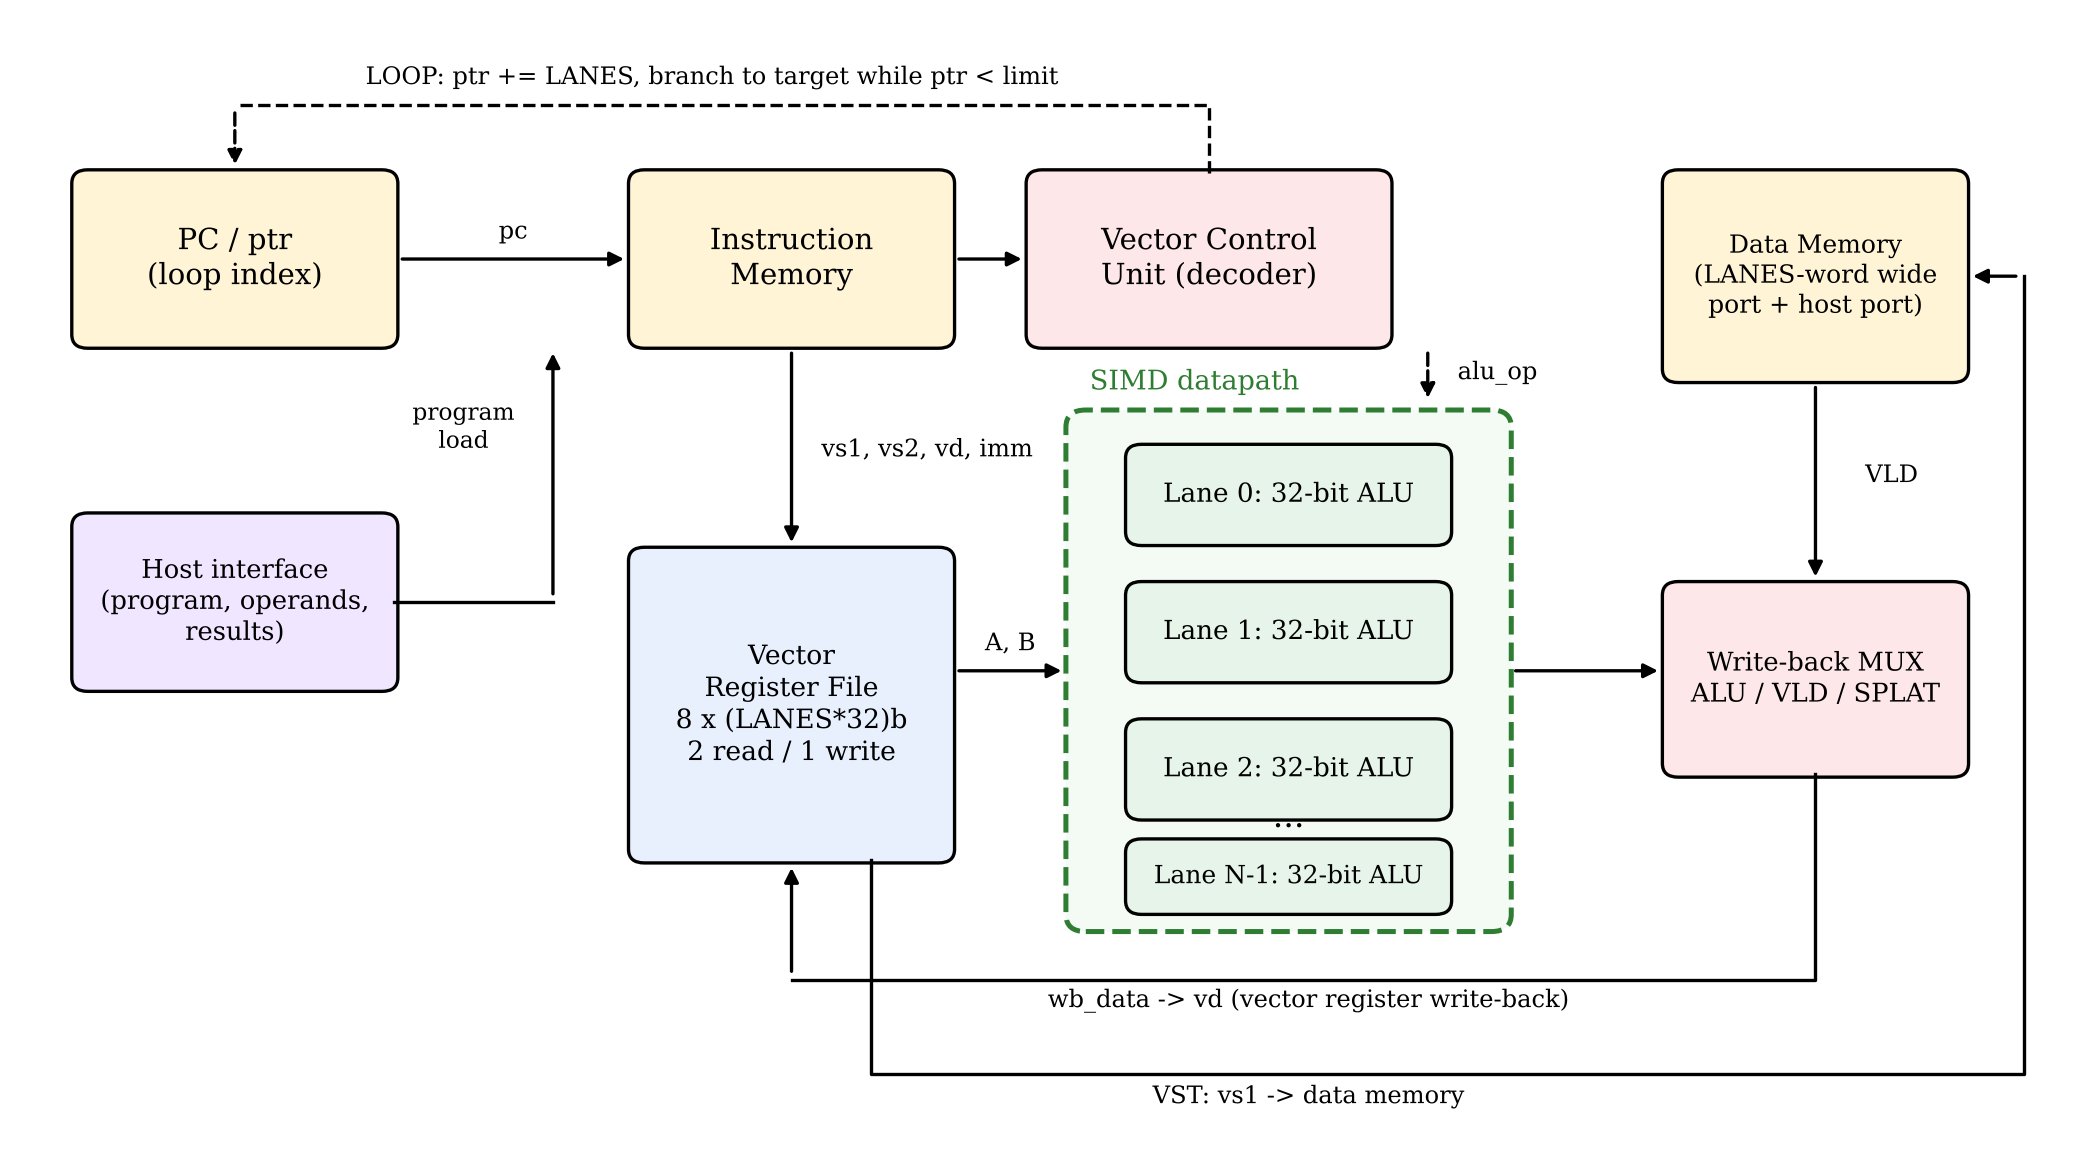
\includegraphics[width=0.9\textwidth]{figures/block_diagram.png}
\caption{Block diagram of the proposed SIMD Vector Processing Unit.}
\label{fig:block}
\end{figure*}

\subsection{Instruction set}
The ISA has sixteen opcodes and a single 32-bit format: opcode [31:28], destination \textit{vd} [27:25], sources \textit{vs1} [24:22] and \textit{vs2} [21:19], and a 19-bit immediate [18:0]. Compare instructions set a lane to all ones (true) or all zeros (false), which allows branch-free conditional selection with a logical AND. Table~\ref{tab:isa} lists the instructions.

\begin{table}[!t]
\caption{Vector Instruction Set}
\label{tab:isa}
\centering
\scriptsize
\renewcommand{\arraystretch}{1.05}
\begin{tabular}{@{}c l p{4.9cm}@{}}
\toprule
\textbf{Op} & \textbf{Mnemonic} & \textbf{Operation (per lane $i$)}\\
\midrule
0 & NOP & No operation\\
1 & VADD & $vd[i]=vs1[i]+vs2[i]$\\
2 & VSUB & $vd[i]=vs1[i]-vs2[i]$\\
3 & VAND & $vd[i]=vs1[i]\ \&\ vs2[i]$\\
4 & VOR & $vd[i]=vs1[i]\ |\ vs2[i]$\\
5 & VXOR & $vd[i]=vs1[i]\oplus vs2[i]$\\
6 & VSLL & $vd[i]=vs1[i]\ll vs2[i][4{:}0]$\\
7 & VSRL & $vd[i]=vs1[i]\gg vs2[i][4{:}0]$ (logical)\\
8 & VMUL & $vd[i]=$ low 32 bits of $vs1[i]\times vs2[i]$\\
9 & VCMPEQ & $vd[i]=(vs1[i]=vs2[i])$ ? all-ones : 0\\
10 & VCMPLT & $vd[i]=($signed $vs1[i]<vs2[i])$ ? all-ones : 0\\
11 & VLD & $vd=\mathit{LANES}$ words at $\mathit{mem}[ptr+imm]$\\
12 & VST & $\mathit{LANES}$ words at $\mathit{mem}[ptr+imm]=vs1$\\
13 & VSPLAT & $vd[i]=$ sign-extended immediate (broadcast)\\
14 & LOOP & $ptr \mathrel{+}= \mathit{LANES}$; if $ptr<limit$ then $pc=target$, otherwise $pc\mathrel{+}{+}$ and clear $ptr$\\
15 & HALT & Stop; freeze counters\\
\bottomrule
\end{tabular}
\end{table}

\subsection{Lane ALU}
Each lane is an independent combinational 32-bit ALU implemented in \texttt{simd\_lane\_alu}. It implements the ten arithmetic, logic, shift, multiply and compare operations of Table~\ref{tab:isa}. Multiplication keeps the low 32 bits of the product, matching wrap-around integer semantics. Because lanes share no state, adding lanes does not lengthen the critical path inside a lane, which is the basis of the scalability observed in Section~\ref{sec:results}.

\subsection{Vector register file and memories}
The register file holds eight vector registers of $\mathit{LANES}\times 32$ bits with two asynchronous read ports and one synchronous write port. The data memory exposes a \textit{LANES}-word-wide port, so one VLD or VST moves a vector per cycle, plus a one-word host port for loading operands and reading results. The instruction memory has a host programming port. Both memories are behavioral models with ideal bandwidth; they are not evidence of a physical block-RAM implementation. Memory timing and bandwidth stalls are outside the current model.

\subsection{Strip-mining loop control}
A conventional scalar loop over $N$ elements would need a counter, a compare and a branch. We instead provide \textit{LOOP target, limit}. Each execution adds \textit{LANES} to \textit{ptr}; if the new value is below \textit{limit} the program counter jumps to \textit{target}, otherwise execution falls through and \textit{ptr} is cleared. All VLD/VST addresses are formed as \textit{ptr} + immediate. Consequently the same program binary, which contains the element count $N$ but not the lane count, runs correctly on any configuration whose lane count divides $N$. This mirrors the lane-agnostic style of SVE and RVV~\cite{stephens2017,rvv2021}.

\subsection{Tool flow and verification}
The RTL is written in Verilog-2005~\cite{verilog2005} and simulated with Icarus Verilog. The directed lane-ALU testbench records 19 passing cases, including wraparound arithmetic, shift boundary values, signed comparison and truncated multiplication. The self-checking system testbench loads programs and operands through host ports, runs each workload to HALT and compares output words against testbench reference values. The checked-in automated results contain four workloads at five lane counts, with zero errors in all 20 configurations. The saved evidence includes simulator logs and a GTKWave-compatible VCD for the four-lane vector-add run.

%=====================================================================
\section{Results and Discussion}
\label{sec:results}
\subsection{Functional verification}
Four workloads were run on each of five lane counts (1, 2, 4, 8, 16), giving 20 system simulations. They are \textit{vadd} ($C=A+B$), \textit{saxpy} ($C=3A+B$), \textit{threshold} ($C=A$ if $A<1000$, else 0) with $N=64$, and \textit{opcover}, which exercises SUB, OR, XOR, SLL, SRL and CMPEQ with $N=16$. All runs finished with zero mismatches. Fig.~\ref{fig:wave} shows a waveform of the four-lane \textit{vadd} run: in cycle 2 the four lanes add their operands in parallel, e.g., \texttt{0xE77A08CE} + \texttt{0x96B1C02D} = \texttt{0x7E2BC8FB} in lane~0, and the result is stored by the following VST. At the end of the first iteration LOOP advances \textit{ptr} from 0 to 4 and returns the program counter to 0.

\begin{figure*}[!t]
\centering
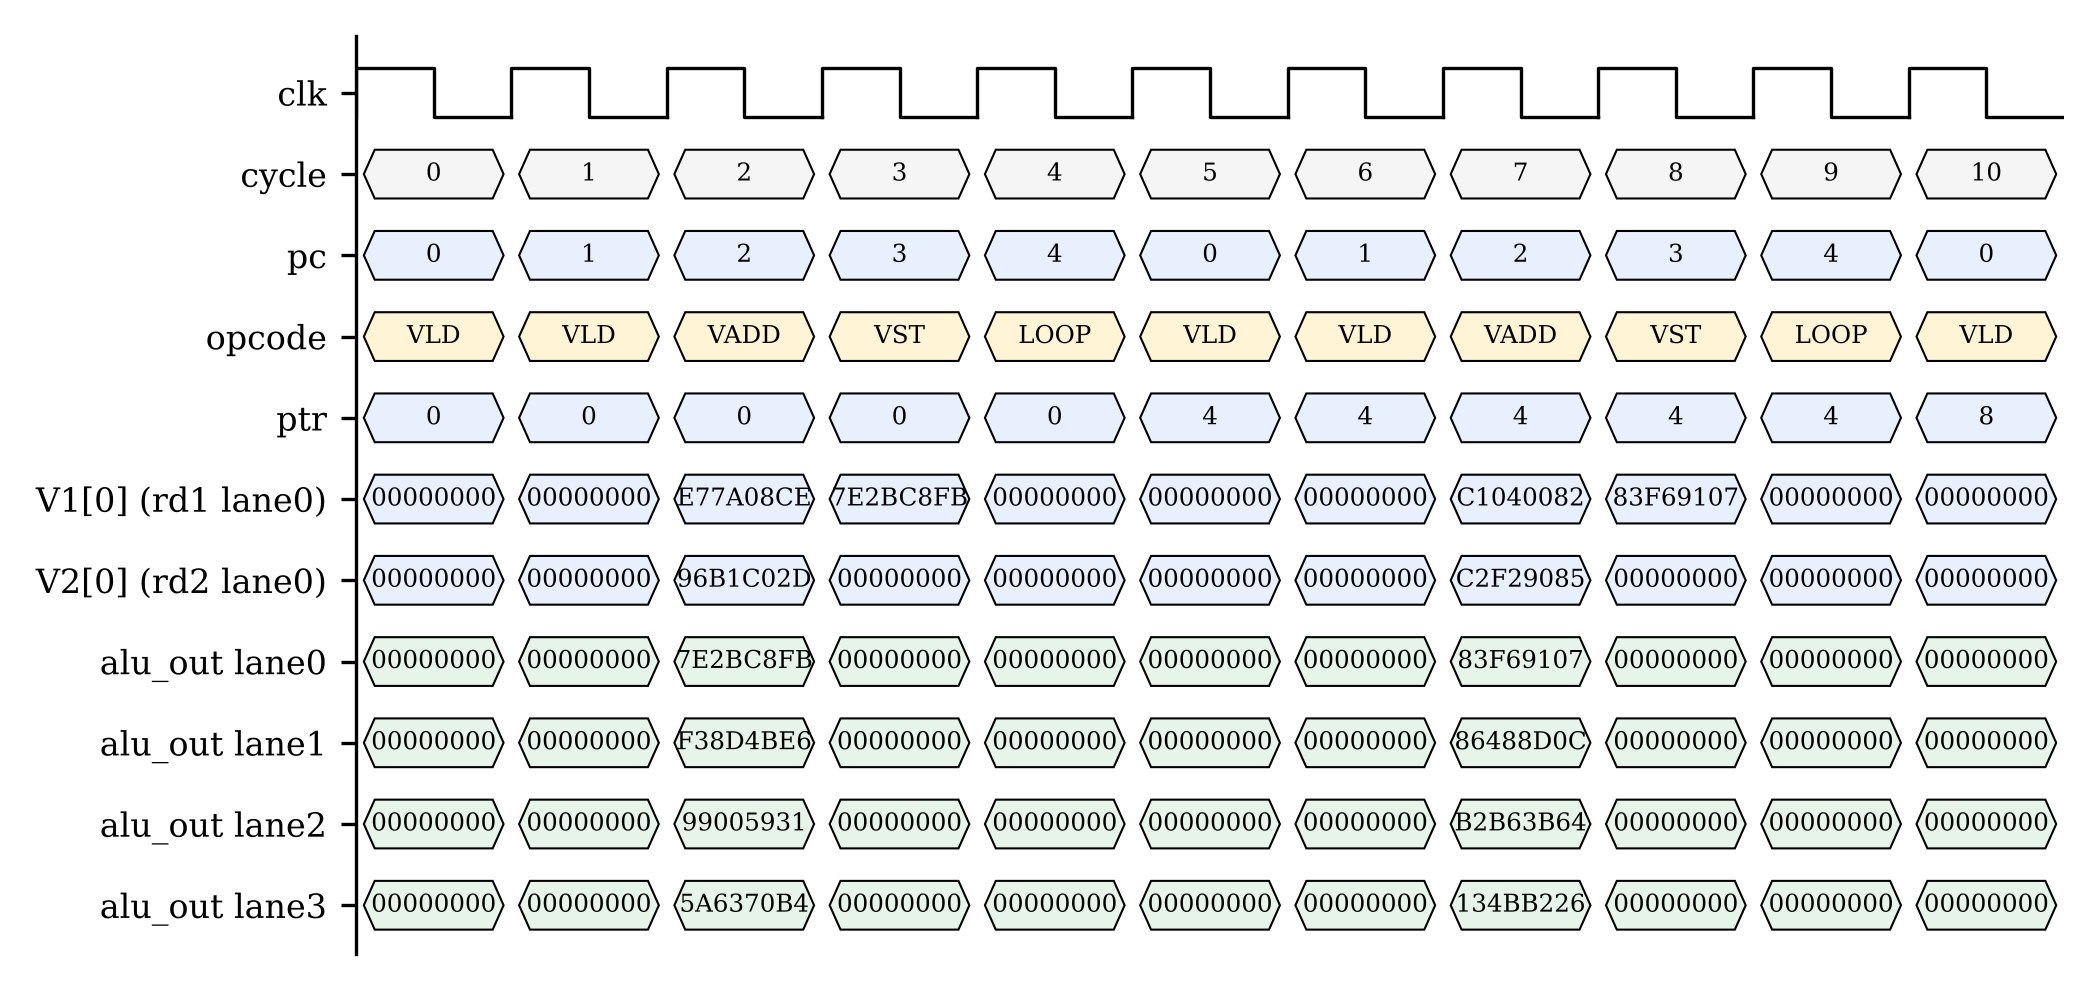
\includegraphics[width=0.92\textwidth]{figures/waveform.png}
\caption{Waveform of the four-lane VPU running vector add, generated from the simulation VCD.}
\label{fig:wave}
\end{figure*}

\subsection{Performance: scalar versus SIMD}
Table~\ref{tab:cycles} gives the cycle count of each workload. The one-lane configuration is the scalar baseline: it executes the identical program on a single ALU, so the comparison isolates the effect of data-level parallelism.

\begin{table}[!t]
\caption{Execution Cycles Versus Number of Lanes}
\label{tab:cycles}
\centering
\small
\begin{tabular}{@{}l c c c c c@{}}
\toprule
\textbf{Workload} & \textbf{1} & \textbf{2} & \textbf{4} & \textbf{8} & \textbf{16}\\
\midrule
vadd      & 321 & 161 & 81 & 41 & 21\\
saxpy     & 386 & 194 & 98 & 50 & 26\\
threshold & 322 & 162 & 82 & 42 & 22\\
opcover   & 241 & 121 & 61 & 31 & 16\\
\bottomrule
\end{tabular}
\end{table}

Because every instruction takes one cycle, cycles equal executed instructions. If the loop body has $k$ instructions (including LOOP), the kernel processes $N$ elements, and $c$ instructions run only once (HALT, plus VSPLAT for SAXPY and threshold), then
\begin{equation}
C(L)=\frac{kN}{L}+c .
\end{equation}
For example, vadd has $k=5$ and $c=1$, giving $5\cdot 64/4+1=81$ cycles on four lanes, exactly as simulated. The speed-up over the scalar baseline is
\begin{equation}
S(L)=\frac{kN+c}{kN/L+c},
\end{equation}
which approaches $L$ for large $kN$, as in Amdahl's law~\cite{amdahl1967} with the one-time instructions acting as the serial fraction. Measured speed-ups are 1.99$\times$ (2 lanes), 3.93--3.96$\times$ (4), 7.67--7.83$\times$ (8) and 14.6--15.3$\times$ (16), see Fig.~\ref{fig:speedup}. The shortfall at 16 lanes comes from the fixed set-up and HALT instructions, which become a larger fraction of a shorter run. These results assume an ideal memory that delivers one full vector per cycle; a real memory hierarchy would reduce the gain for bandwidth-bound kernels and is a limitation of the present prototype.

\begin{figure}[!t]
\centering
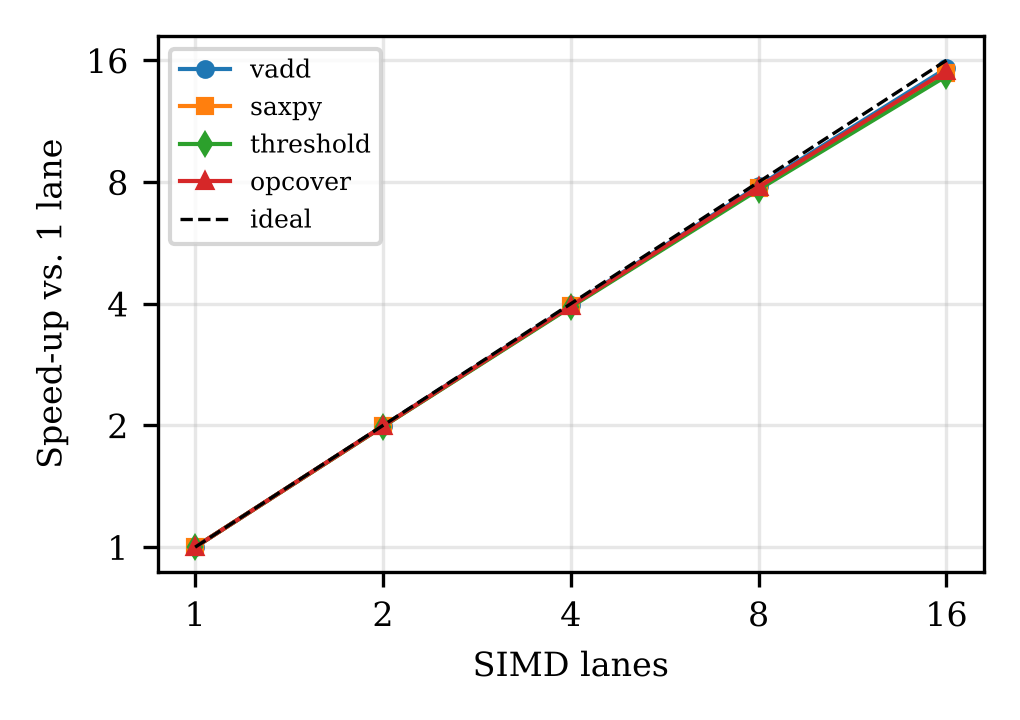
\includegraphics[width=0.92\columnwidth]{figures/speedup.png}
\caption{Measured speed-up over the one-lane baseline.}
\label{fig:speedup}
\end{figure}

\subsection{Synthesis results}
The saved Yosys runs use Xilinx 7-series mapping on separate RTL modules. The lane-ALU report contains 503 LUT cells in total (the sum of LUT2--LUT6), three DSP48E1 cells, 19 CARRY4 cells, 30 MUXF7 cells and 15 MUXF8 cells. The control report contains six LUT4 cells. Separate vector-register-file reports contain 12, 22, 44 and 86 RAM32M cells for 1, 2, 4 and 8 lanes, respectively. These module results are summarized in Table~\ref{tab:synth}; they are not additive top-level VPU utilization because the ALUs, memories, host logic and interconnect were not synthesized together. The standalone module statistics also include mapping details such as I/O buffers and are not a placed design-level utilization report. The saved flow does not report a target device, timing constraints, place-and-route utilization or maximum frequency. Accordingly, no FPGA fit or clock-rate conclusion is made.

\begin{table}[H]
\caption{Saved Yosys Statistics for Selected RTL Modules}
\label{tab:synth}
\centering
\small
\scriptsize
\setlength{\tabcolsep}{3pt}
\begin{tabular}{@{}p{2.1cm} c c c p{2.7cm}@{}}
\toprule
\textbf{Module} & \textbf{LUT} & \textbf{DSP48E1} & \textbf{RAM32M} & \textbf{Other mapped cells}\\
\midrule
Lane ALU & 503 & 3 & --- & 19 CARRY4; 30 MUXF7; 15 MUXF8\\
Control & 6 & 0 & --- & LUT4\\
Vector RF, 1 lane & --- & 0 & 12 & ---\\
Vector RF, 2 lanes & --- & 0 & 22 & ---\\
Vector RF, 4 lanes & --- & 0 & 44 & ---\\
Vector RF, 8 lanes & --- & 0 & 86 & ---\\
\bottomrule
\end{tabular}
\end{table}

\subsection{Limitations}
The implementation is a single-cycle educational datapath with an ideal vector-wide behavioral memory model. It is not a five-stage pipelined CPU and has no hazard detection or forwarding, cache or TLB, multicore coherence, GPU SIMT, vector masks or sub-word elements. The cycle comparisons therefore describe this simulator model and do not predict wall-clock latency on an FPGA. The project brief includes resource utilization and maximum-frequency analysis; the current saved synthesis covers selected modules only, and maximum frequency remains unmeasured.

%=====================================================================
\section{Individual Contributions}
Member labels M1--M4 follow the title-page order. Table~\ref{tab:matrix} records the documented contributions; $\bullet$ marks primary responsibility and $\circ$ marks supporting work or review.

\begin{table}[H]
\caption{Contribution Matrix ($\bullet$ = primary responsibility, $\circ$ = support or review)}
\label{tab:matrix}
\centering
\scriptsize
\renewcommand{\arraystretch}{1.12}
\setlength{\tabcolsep}{3.5pt}
\begin{tabular}{@{}p{3.55cm} c c c c@{}}
\toprule
\textbf{Task} & \shortstack{\textbf{M1}\\Yaseen} & \shortstack{\textbf{M2}\\Palwai} & \shortstack{\textbf{M3}\\Nishant} & \shortstack{\textbf{M4}\\Sankalp}\\
\midrule
ISA definition, control unit              & $\bullet$ & $\circ$   &           &           \\
Top level, PC and LOOP logic              & $\bullet$ &           & $\circ$   &           \\
Lane ALU and directed unit test           & $\circ$   & $\bullet$ &           &           \\
Vector register file                      &           & $\bullet$ & $\circ$   &           \\
Memories and host interface               & $\circ$   &           & $\bullet$ &           \\
Assembler and workloads                   &           &           & $\bullet$ & $\circ$   \\
System testbench and CI        & $\circ$   & $\circ$   & $\bullet$ &           \\
Synthesis estimates                       &           & $\circ$   &           & $\bullet$ \\
Figures and result analysis                & $\circ$   &           & $\circ$   & $\bullet$ \\
IEEE report (own sections)                 & $\bullet$ & $\bullet$ & $\bullet$ & $\bullet$ \\
Prototype video (own segment)              & $\bullet$ & $\bullet$ & $\bullet$ & $\bullet$ \\
Repository, README, docs                   & $\circ$   &           & $\circ$   & $\bullet$ \\
\bottomrule
\end{tabular}
\end{table}

M1 defined the instruction set and implemented the control unit and top level; M2 implemented the lane ALU, vector register file and directed ALU test; M3 implemented the memories and host interface, assembler, workloads and system-level verification flow; and M4 generated the synthesis estimates, result figures and analysis, and project documentation. The report and prototype demonstration include contributions from all four members.

%=====================================================================
\section{Conclusion}
The project delivers a parameterized Verilog SIMD VPU, a defined vector ISA, an assembler, self-checking testbenches and saved simulation and synthesis evidence. Across four workloads and five lane counts, all 20 saved system configurations report zero errors; the directed ALU test reports 19 passing cases. Four-lane vector addition completes in 81 cycles versus 321 cycles for the one-lane baseline, a 3.96$\times$ cycle-count speed-up. The evidence demonstrates correct lane-parallel operation and increasing cycle-level throughput under the behavioral memory model. Since the saved Yosys reports cover separate modules and no FPGA timing flow is available, whole-device resource use and maximum frequency remain open measurements.

\bibliographystyle{IEEEtran}
\bibliography{references}

\end{document}
